\section{Technologies}
The development of the web application went through multiple iterations before settling on the current choice of technologies used. The application uses the JavaScript library React for the frontend user interface with the Material UI library for components, and the Python web framework Flask for the backend algorithms with PyPy for faster runtimes. This section discusses the decisions made when choosing the main technologies (frameworks, libraries etc).

\subsection{Initial Ideas}
 The software was initially planned to be a local Python only application, using the Tkinter GUI library. This was because the author is most familiar with the Python programming language, and has some limited experience with the Tkinter library. However, early prototypes of this software using Tkinter proved to be cumbersome to work with and have a dated visual style. Alternative Python UI libraries (such as PyQt and Kivy) were also considered, but proved to have learning curves no steeper than using an entirely different language.
 
\begin{figure}[h]
    \centering
    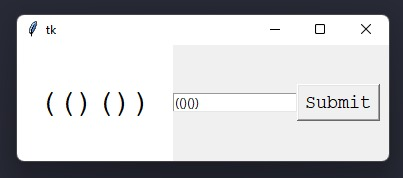
\includegraphics[scale = 0.7]{./images/tkinter-gui.jpeg}
    \caption{An early iteration of the software using Tkinter}
\end{figure}

We then considered the prospect of a web application; the author again had some limited experience with HTML/CSS, but using these languages to control the layout and sizing of the UI seemed much more intuitive. This approach also naturally allowed for separation between the UI and the strategies, and the author's familiarity with Python could still be leveraged as a backend language. The author had also wished to learn the technologies used for web development, so this seemed like the natural approach to take.

\subsection{Backend}
The strategies to run on Dyck words are implemented in Python but run using PyPy, and communicated with the frontend using Flask.

\subsubsection{Flask}
Flask is a web framework that allows users to build a web server with Python that they can communicate with using HTTP requests, allowing Python to be used as a backend language \cite{whatisFlask}. One of the reasons Flask was chosen over potential alternatives, such as Django, is due to its simplicity. Flask is classed as a microframework, meaning it does not have a lot of dependencies or libraries required to use it. This makes Flask fairly lightweight and efficient for our purposes, reducing overhead when communicating requests back and forth. 

\begin{figure}[h]
    \centering
    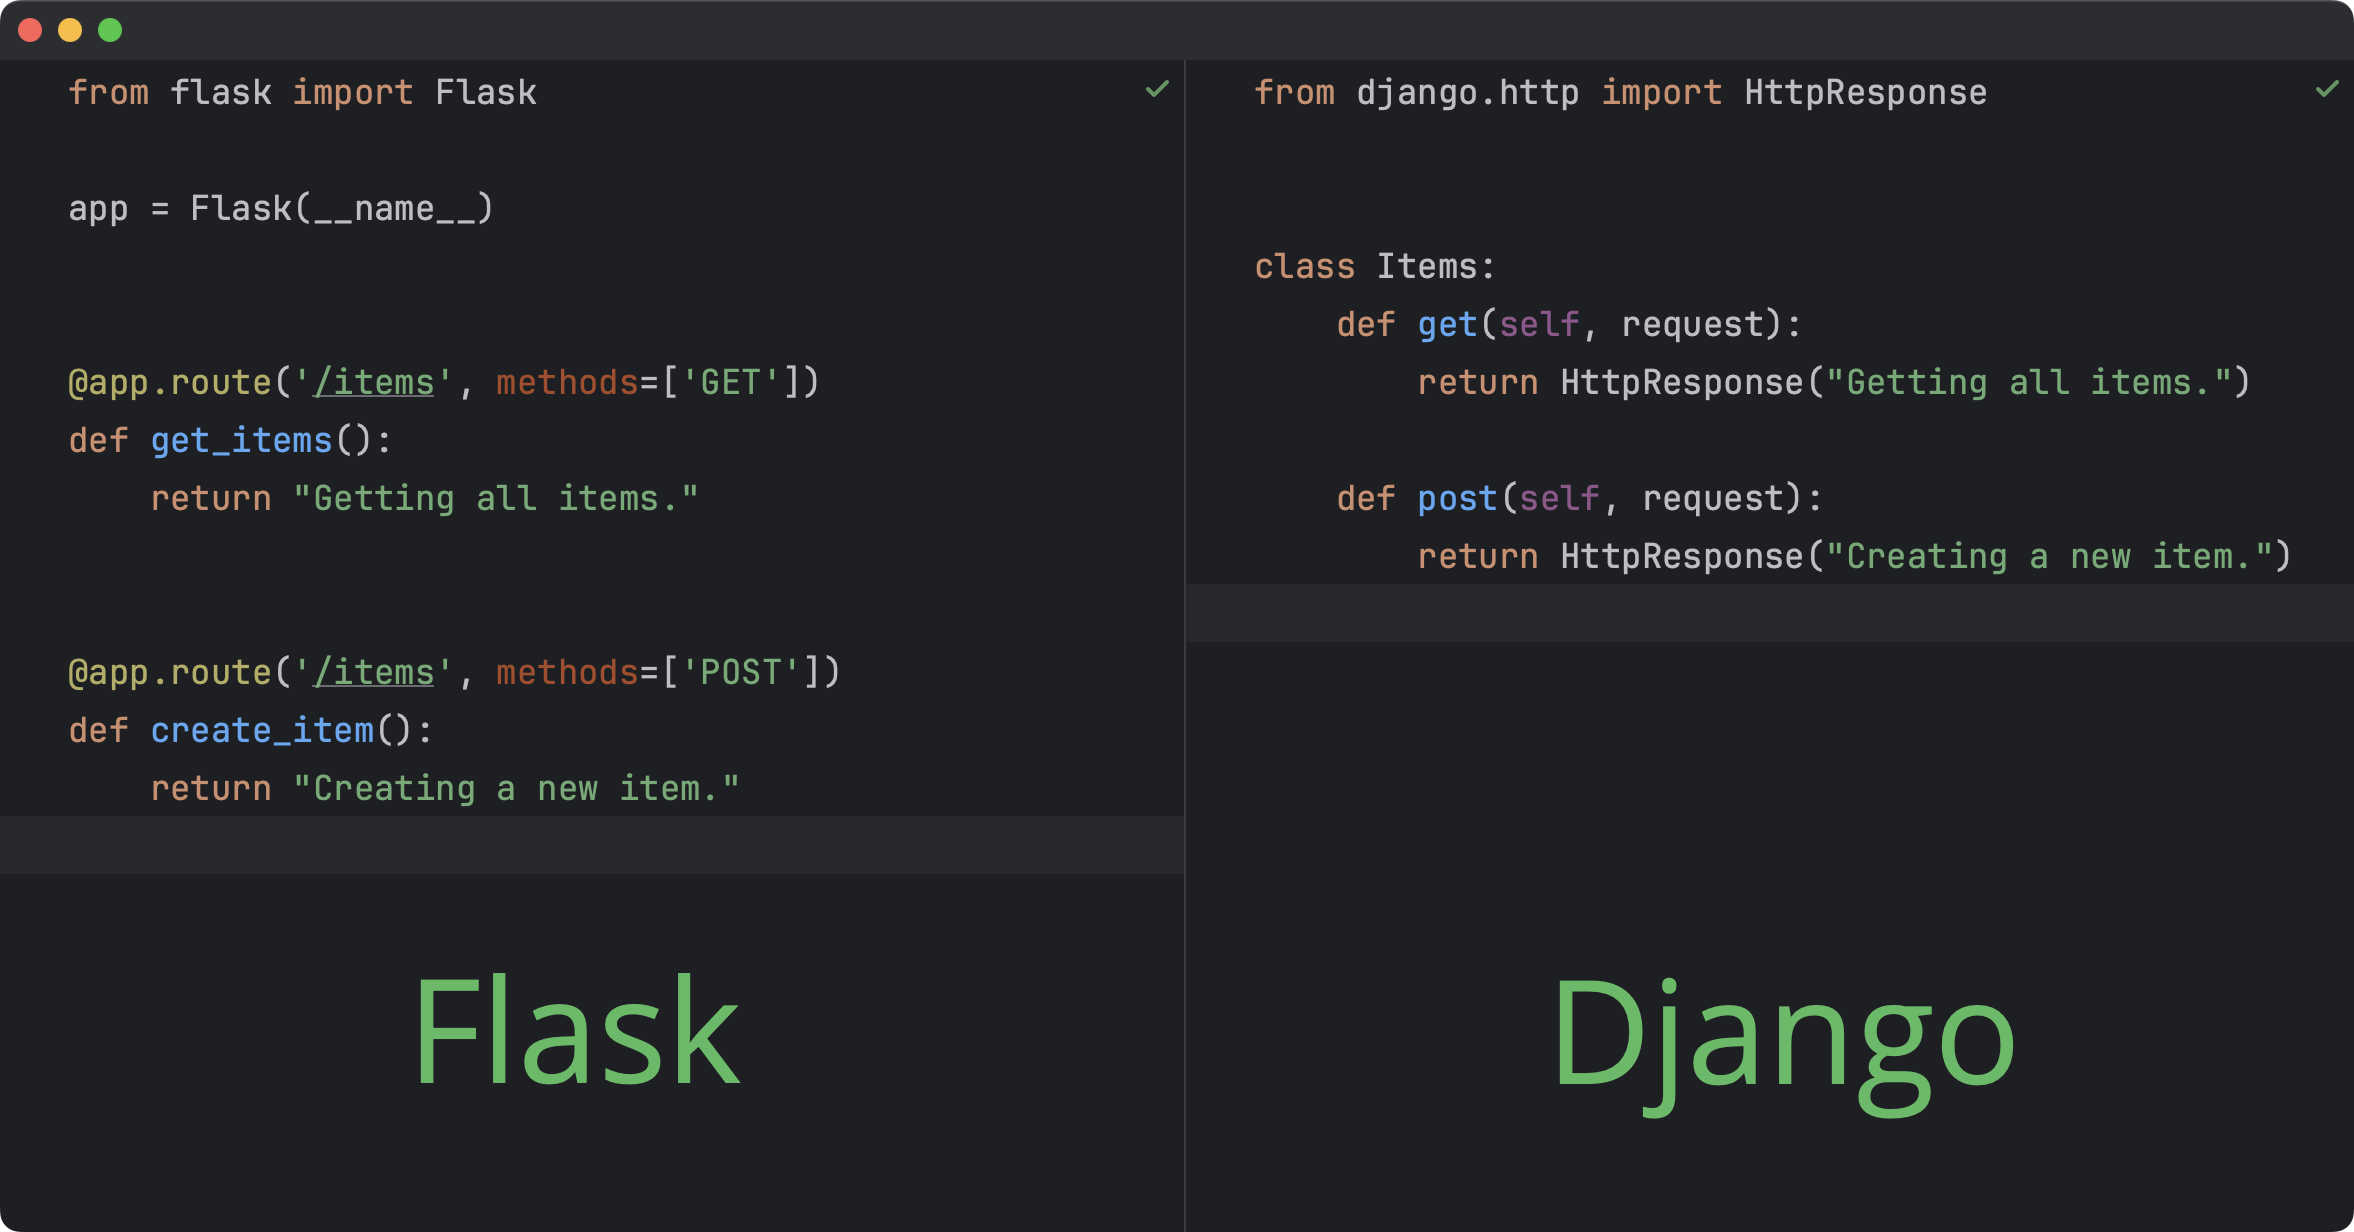
\includegraphics[scale=0.3]{./images/flaskVSdjango.png}
    \caption{Implementing the same functionality in Flask and Django \cite{flaskVSdjango}}
\end{figure}

Figure 3.2 shows the difference between using Flask and Django. In the Flask example, the same functions could be used with the only modification being an app route, which is added directly above the function. This binds each function to the route URL plus its given route, and depending on the type of request either ``get\textunderscore~items()'' or ``create\textunderscore~items()'' would be called. Thus, any work done to translate a re-pairing strategy into an algorithm could easily be implemented using Flask by simply adding an app route at the top.

\subsubsection{PyPy}
During the implementation of the web application, the author discovered PyPy. This is an alternative implementation of Python, providing faster execution times and less memory usage than the standard implementation.

In particular, PyPy uses a Just-In-Time compiler, which converts Python code into machine code at runtime. This makes PyPy have the greatest speed-up when executing long-running programs where a significant fraction of the time is spent executing Python code \cite{whatisPyPy}, which is exactly what the backend will be doing (particularly when brute forcing for the width of a Dyck word). 

Exceution of the program below, which computes the factorial of 20000 and repeats this 500 times, demonstrates the potential speed-up that PyPy can provide:

\begin{figure}[h]
    \centering
    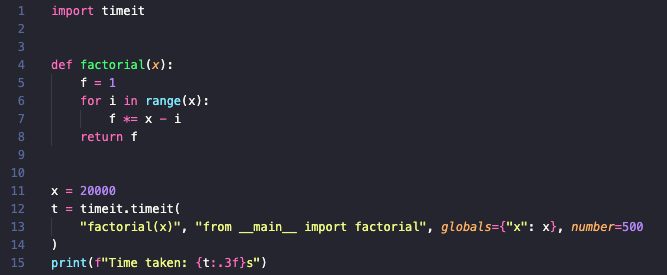
\includegraphics[scale=0.55]{./images/factorialPyPy.png}
    \caption{Computes 20000! 500 times}
\end{figure}

Executing this program using Python takes 77.930s, but using PyPy takes 31.872s. The program also requires no modifications to run on PyPy, since PyPy is a restricted subset of Python called RPython. However, these restrictions have had no impact on the development of this web application.

All of the re-pairing strategies (Simple, Non-Simple, Simple Greedy) were trivial implementations into algorithms due to the nature of Python's syntax.


\subsection{Frontend}

\subsubsection{React}
Naturally, the components of the UI would need ways of interacting with one another. This led to using React, which is a JavaScript library used to simplify the process of creating user interfaces \cite{whatisReact}. It allows modular user interface components to be built, and later nested and combined to create a dynamic and interactive webpage. 

The web application is designed as a single page application (SPA), meaning it loads only a single web document and updates its contents dynamically. In contrast, typical websites will make the web browser load entire new pages when the contents of the page need to be modified \cite{singlepageapp}. React fits the development of SPAs well, since each component has its own state and properties, and React will only automatically re-render components if there is a change to one of these.
This allows for greater performance gains due to the lower overhead and a more dynamic experience.

\subsubsection{Material UI}
 Rather than styling the components of the web application from scratch, the author opted to use Material UI. This is a React component library that implements the design language made by Google, and contains a collection of prebuilt components with customisation options.

\begin{figure}[h]
    \centering
    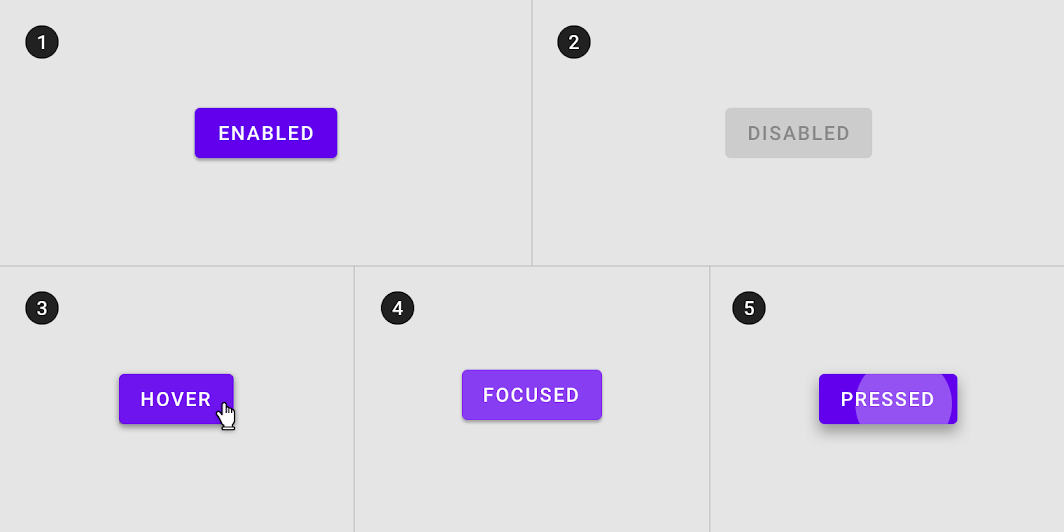
\includegraphics[scale=0.35]{./images/materialUIbutton.png}
    \caption{An example of how a Material UI button varies depending on its state \cite{materialUIbuttons}}
\end{figure}

\subsubsection{Javascript}
Why do we use JS over TS?